\chapter{Analysis}\label{sec:analysis}
The current treemap implementation and its set of possible interactions is described in Section~\ref{sec:analysis:existing-interactions}.
For the implementation of the \gv{} several web frameworks are compared and advantages and disadvantages are contrasted in Section~\ref{sec:analysis:frontend-framework-comparison}.

Section~\ref{sec:analysis:examples} describes essential characteristics of interactions in single and multiple data visualizations.
These characteristics are relevant for a formalized language of \cmvs{}.
To accomplish this goal, the approach is to deduce the characteristics by a list of examples.
What are the expected data structures for each visualization?
Which visual variables can be used to show the effect of an interaction?
A list of possible interactions is given for each visualization.
Those interactions will be classified according to \textcite{Yi2007} and the relevant subject of the interaction is specified.



\section{Existing Interactions}\label{sec:analysis:existing-interactions}
The current implementation comes with a visualization of a \tmap{} and should be complemented with a \gv{}.
In this section, the set of already possible interactions are classified according to \textcite{Yi2007} as in Section~\ref{sec:related-work:interaction-theory:categories}.
They fall into these categories: \emph{select}, \emph{explore}, \emph{reconfigure}, \emph{encode} and \emph{filter}.

The user can \emph{select} one item in the view by clicking on it.
The user can reveal a tooltip showing the item properties by moving the mouse cursor on the item, which is another \emph{select} interaction.

The user can \emph{explore} the map in the usual manner:
If the user drags with the mouse on the map, a panning operation is performed with the viewpoint focused on the \tmap{}, like a turntable.
The zoom factor can be changed by scrolling with the mouse on the canvas of the map.

\emph{Encode} and \emph{reconfigure} techniques are performed through a menu:
The user can \emph{reconfigure} different data sets and the displayed diagram, e.g.\ a treemap visualization based on the geometry shape, cubes or voronoi regions.
In a sub-menu the user can \emph{encode} properties of a data set in predefined visual variables, e.g.\ the height, color and texture of an item.
A slider can be used to \emph{filter} the data set on a data attribute.
When the user drags the slider and changes an upper or a lower limit, items with an attribute beyond this interval are filtered out.



\section{Requirements for Coordinated Multiple Views}\label{sec:analysis:requirements}
The existing implementation should be complemented with a coordinated multiple view layout.
Next to the \tmap{} a \gv{} should appear, so that the user can understand the geographic context of items in the treemap.

To ensure a future use of the software, this section provides a list of software requirements.
Later in Chapter~\ref{sec:evaluation} these requirements will be reused to evaluate the system.

\begin{enumerate}
  \item Serialization

    Serialization is the process of translating objects that can be stored or transmitted and reconstructed later.
    In order to coordinate interactions among views, information needs to be passed from one view to another.
    A framework for \cmvs{} should therefore find a serialization format for interactions which has
    \begin{enumerate*}[label=(\arabic*)]
      \item
        small payloads and
      \item
        fast serialization and deserialization.
    \end{enumerate*}

  \item Reversibility

  Reversibility means, in the context of \cmvs{}, the ability to undo the effect of an interaction.
  Ideally, every interaction should be undoable.
  If not every interaction is undoable, the cost to replay the interactions from the original state up to the point of the interaction should be minimized.

\item Software Extensibility

  Software extensibility means, in this thesis, the costs of changing behaviour.
  How many views need to be touched, if a new interaction option is added to the system?
  How much time and effort is necessary to implement the new feature?

\item Maintainability

  Maintainability means, in this thesis, the costs of changing the source code.
  How error-prone is the system, will other views be affected if a new interaction is added to the system?

\end{enumerate}



\section{Component pattern and Web Frameworks}\label{sec:analysis:frontend-framework-comparison}

The current \visan{} is a web application and the complementing \gls{cmv} extension should be based on web technologies, too.
Many popular web frameworks like Angular, Ember, React and Vue have developed mechanisms to update UI elements during user interactions.
Because a view in a \cmv{} is a UI element as well, it is worth to consider one of these web frameworks for the implementation of the \cmv{}.

One software pattern, which is a commonly used update mechanism e.g.\ in Ember and React, is the so-called ``component'' pattern.
It has become so widespread and prevalent that it triggered even a web specification called “web components”.
This section evaluates the most suitable component based JavaScript framework for \cmvs{} and whether or not to follow the ``web components'' web specification.

Three JavaScript frameworks have been evaluated:
\begin{enumerate*}[label=(\arabic*)]
  \item GlimmerJS
  \item Google Polymer and
  \item ReactJS.
\end{enumerate*}
GlimmerJS is the templating engine of Ember, the framework which the author of this thesis is most familiar with.
Applications written with GlimmerJS can be built and exported as web components.
Google Polymer is the most popular framework for web components.
React is another very popular framework developed by Facebook, but does not support web components at all.

Most importantly, \cmvs{} require a way to exchange data between views, which is specific to interactions.
The web component specification, unfortunately, does not specify how arbitrary JavaScript objects can be passed to web components.
String based attributes are supported, as seen in Listing~\ref{lst:evaluation:web-components-data}.

To pass rich data to components however, web component frameworks have to roll their own data flow and syntax.
Google Polymer's own syntax to pass rich data to a components is shown in Listing~\ref{lst:evaluation:polymer-data}.
But this is a custom solution that abandons standard HTML.


\lstinputlisting[
  language=HTML,
  label={lst:evaluation:web-components-data},
  caption={An example of string based attributes of web components~\parencite{GoogleMapWebComponent2017}.}
]{listings/evaluation/web-components-data.html}

\lstinputlisting[
  language=HTML,
  label={lst:evaluation:polymer-data},
  caption={An small syntax example how Google Polymer passes rich data to a component.}
]{listings/evaluation/polymer-data.html}

This raises some problems in existing applications:
A particular component-based frontend framework can not be assumed, a lot of existing applications are also written without any JavaScript framework.
Custom solutions like the one of Polymer reduce the main motivation of implementing against web components:
Platform agnostic flexibility.

As a summary, if there is
\begin{enumerate*}[label=(\arabic*)]
  \item no obligation to implement web components and
  \item an easy integration into an existing application is necessary,
\end{enumerate*}
then React is the perfect choice for \cmvs{}.

Table~\ref{tab:implementation:frontend-frameworks} shows the pros and cons of each framework for the use case.

\begin{table}
  \caption{Comparison of component based web frameworks, advantages highlighted in green, disadvantages highlighted in red.}
  \label{tab:implementation:frontend-frameworks}
  \begin{tabularx}{\linewidth}{a a a}
\hline
    \mc{2}{Web Components} & \mc{1}{Specific Framework}  \\
\hline
    \cellcolor{lightgreen}{standard} & \cellcolor{lightred}{string-based attributes} &  \cellcolor{lightred}{no standard}   \\
\hline
    \mc{1}{GlimmerJS} & \mc{1}{Google Polymer} & \mc{1}{React} \\
\hline
  familiarity &  maturity &  maturity \\
  &  documentation   & documentation  \\
  &  community & large community \\
  &  & declarative style  \\
  &  & small size         \\
  &  & integrability      \\
\hline
\hline
\end{tabularx}
\end{table}

\section{Arbitrary Data Visualization Techniques}\label{sec:analysis:examples}

Even though the use case of the \cmv{} is focused on a \tmap{} and a \gv{}, the implementation should allow any kind of data visualizations to be added and coordinated as well.
Instead of implementing as many data visualizations as possible, the approach in this thesis is to analyse many data visualization techniques theoretically.
The goal is to come up with a set of formal requirements and a specification that anticipates additional data visualizations.
With regard to the software requirements in Section~\ref{sec:analysis:requirements}, the \cmv{} framework needs to be extensible and maintainable.

The data visualization catalogue by Severino Ribecca lists many of the most used data visualizations~\parencite{VisualizationCatalogue2017}.
This section covers a selection of data visualization techniques from that catalogue.
For each technique the expected data structure is examined and a list of plausible interactions is systematically analysed.
The gathered knowledge is a preparation of the conceptual framework in Section~\ref{sec:concept}.

\subsection{Line Graphs}
\begin{figure}
  \begin{center}
    \subfloat[Line graphs]{{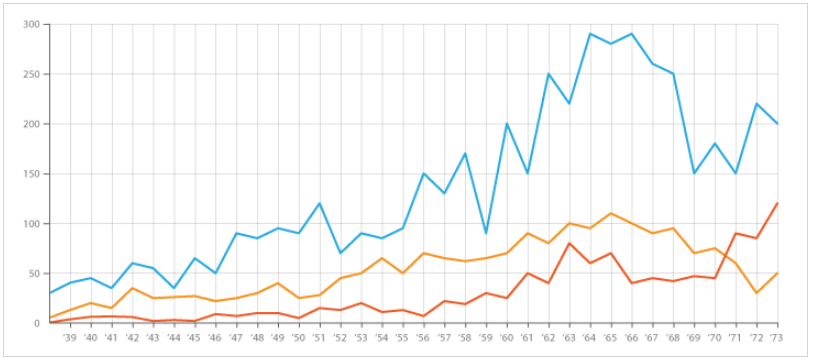
\includegraphics[width=0.4\linewidth]{figures/analysis/line-graphs} }}%
    \qquad
  \caption{Line graphs are used to display trends.}
  \label{fig:analysis:line-graphs}
  \end{center}
\end{figure}

Line graphs display how quantitative values have changed over time.
You can see an example in Figure~\ref{fig:analysis:line-graphs}.
They are perfectly suited to show trends or compare multiple series of data with each other.
Line graphs visualize one or many series of data in parallel and therefore the expected data format is \emph{tabular}.

Line graphs are drawn in a Cartesian coordinate system, connecting subsequent points to each other.
Thus,
\begin{enumerate*}[label=(\arabic*)]
    \item position
    \item orientation and
    \item texture
\end{enumerate*}
are constrained by the visualization technique.
However, an interaction with the line graph can alter the
\begin{enumerate*}[label=(\arabic*)]
    \item shape
    \item color or
    \item size
\end{enumerate*}
of lines to communicate an interaction.
It is further possible to highlight either the entire series of data or a single data point within that series, e.g. changing the shape and size of the point.
Table~\ref{tab:analysis:line-graph:interactions} shows a list of plausible interactions in a line graph.

\begin{table}[H]
  \centering
  \caption{Plausible interactions for line graphs.}%
  \label{tab:analysis:line-graph:interactions}
  \begin{tabularx}{\linewidth}{lXX}
    \bf Category & \bf Description & \bf Required information \\
    \hline
    Select & Highlight a data point & id of data point \\
    Select & Highlight a data series & id of data series \\
    Encode & Change colours of data series & id of data series + colour \\
    Filter & Restrict interval on x-axis & lower limit + upper limit \\
    Filter & Hide a data series & id of data series \\
  \end{tabularx}
\end{table}




\subsection{Bar Charts and Multi-Set Bar Charts}

\begin{figure}
  \begin{center}
    \subfloat[Bar Chart or column graph]{{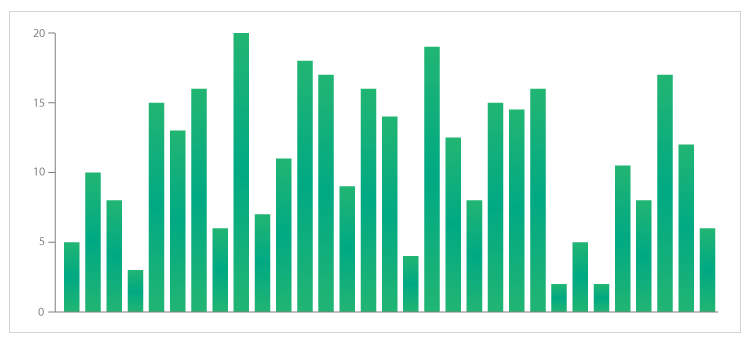
\includegraphics[width=0.4\linewidth]{figures/analysis/bar-chart} }}%
    \qquad
    \subfloat[Multi set bar Chart]{{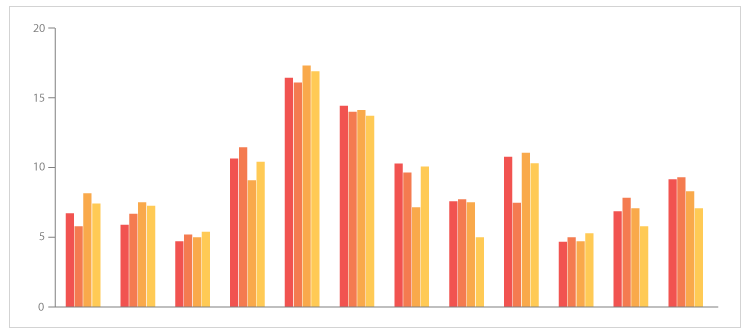
\includegraphics[width=0.4\linewidth]{figures/analysis/multiset-bar-chart} }}%
    \caption{A multi set bar charts is a variation of a bar chart~\parencite{VisualizationCatalogue2017}.}
    \label{fig:analysis:bar-charts}
  \end{center}
\end{figure}

Bar charts use either horizontal or vertical bars to show discrete, numerical comparisons across categories.
The length of a bar displays a quantitative value of a category.
You can see two examples in Figure~\ref{fig:analysis:bar-charts}.

Multiple bar charts display many data series next to each other.
Every series is grouped by category and a colour can be used to identify a data series.
Like line graphs, bar charts expect a \emph{tabular} data format.
In contrast to line graphs, bar charts are used to show a comparison rather than a trend.

The type of the visualization constrains the
\begin{enumerate*}[label=(\arabic*)]
    \item shape,
    \item size and, in case of a multi set bar charts,
    \item the colour
\end{enumerate*}
of the visualization.
An interaction can be shown by altering
\begin{enumerate*}[label=(\arabic*)]
    \item position,
    \item colour,
    \item shape and
    \item the texture
\end{enumerate*}
of bars and columns.
Table~\ref{tab:analysis:bar-charts:interactions} lists some possible interactions.


\begin{table}[H]
  \centering
  \caption{Plausible interactions for bar charts.}
  \label{tab:analysis:bar-charts:interactions}
  \begin{tabularx}{\linewidth}{lXX}
    \bf Category & \bf Description & \bf Required information \\
    \hline
    Select & Highlight a bar & id of data point \\
    Encode & Change colours of data series & id of data serie(s) + colour(s) \\
    Reconfigure & Sort by attribute & name of data attribute \\
    Reconfigure & Drag bars to reorder data series & ordered list of ids of data series \\
    Filter & Hide a data series & id of data series \\
  \end{tabularx}
\end{table}

\subsection{Histograms}

\begin{figure}
  \centering
  \subfloat[Histogram]{{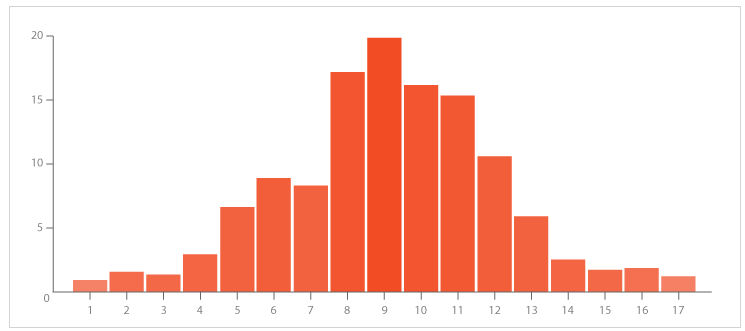
\includegraphics[width=0.4\linewidth]{figures/analysis/histogram} }}%
  \qquad
  \subfloat[Population Pyramid]{{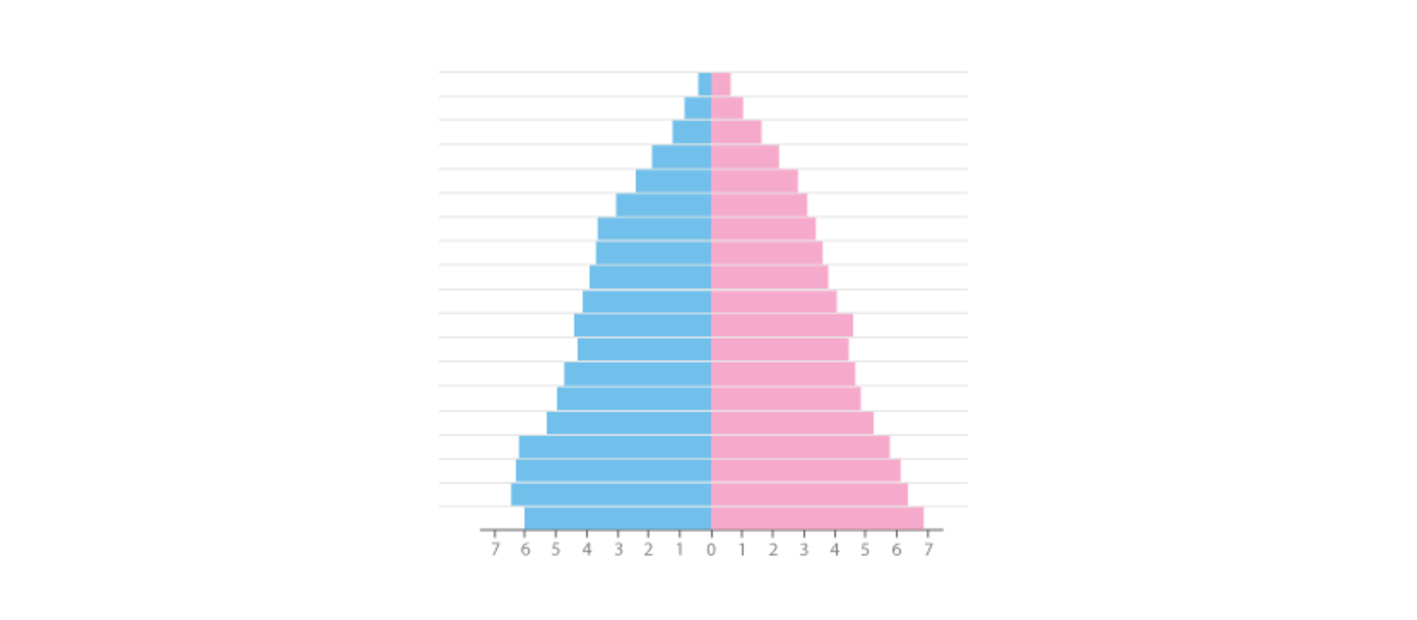
\includegraphics[width=0.4\linewidth]{figures/analysis/population-pyramid} }}%
  \caption{A histogram is a bar chart over a continuous interval~\parencite{VisualizationCatalogue2017}.}%
  \label{fig:analysis:histograms}
\end{figure}

Histograms, as shown in Figure~\ref{fig:analysis:histograms}, visualize the distribution of data over a continuous interval or a certain time period.
A special type is the population pyramid, which is a pair of back-to-back histograms, one for each sex.

Histograms and bar charts expect the same kind of data, i.e.\ a \emph{tabular} data structure.
Almost the same interactions as in Table~\ref{tab:analysis:bar-charts:interactions} can be applied to histograms, except a re-ordering of bars along the x-axis.
This is not possible, because the histogram constrains the position of bars along the interval.

\subsection{Bubble Charts and Scatter Plots}

\begin{figure}
  \centering
  \subfloat[Bubble Chart]{{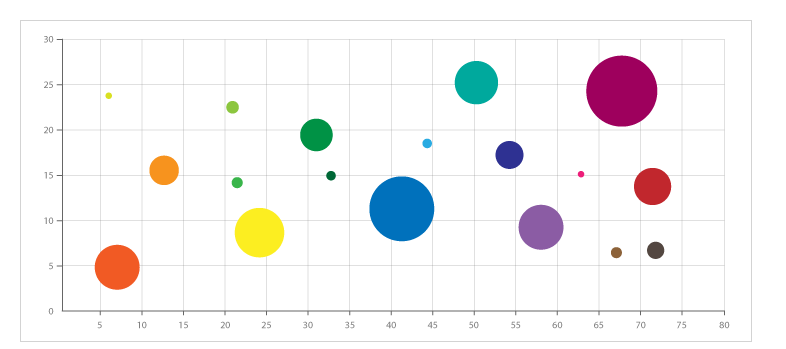
\includegraphics[width=0.4\linewidth]{figures/analysis/bubble-chart} }}%
  \qquad
  \subfloat[Scatter plot]{{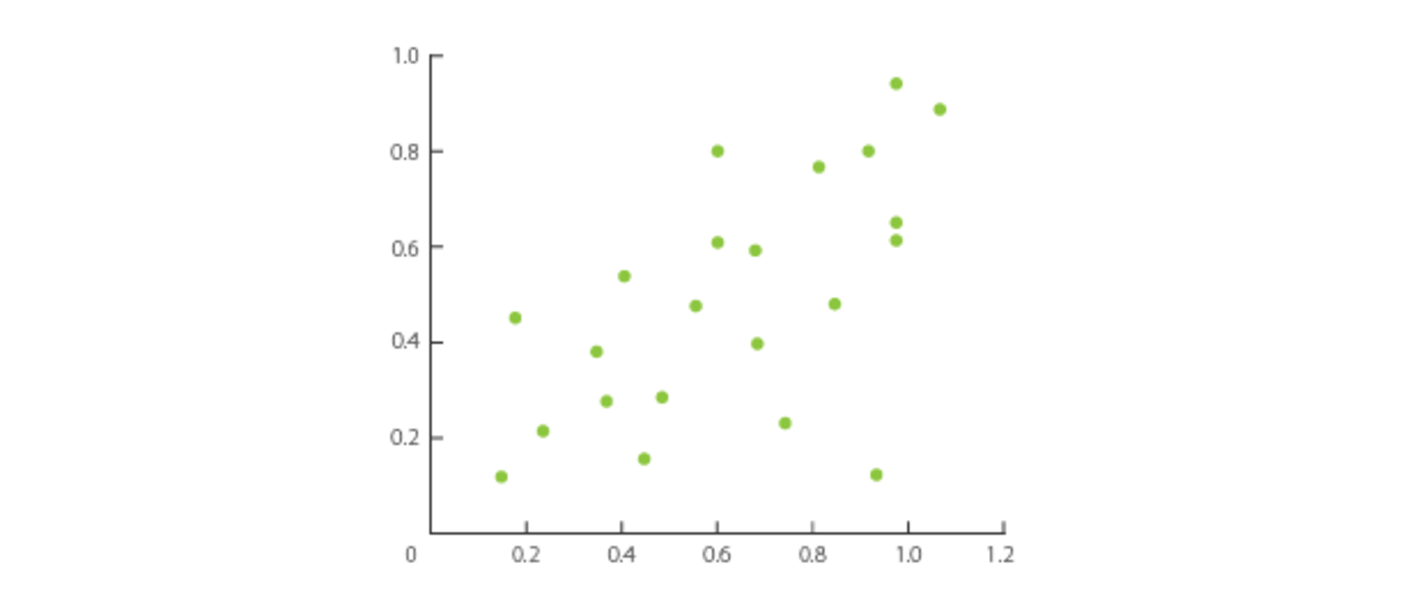
\includegraphics[width=0.4\linewidth]{figures/analysis/scatter-plot} }}%
  \caption{Bubble charts and scatter plots are similar regarding interactions~\parencite{VisualizationCatalogue2017}.}%
  \label{fig:analysis:bubble-chart}
\end{figure}

Both bubble charts and scatter plots are techniques to visualize continuous values from two data attributes.
Points are placed with the two attributes in Cartesian coordinates in order to detect relationships and correlations.
An example for each technique is displayed in Figure~\ref{fig:analysis:bubble-chart}.

In case of bubble charts, each point is displayed as a bubble with a third value encoded in the size of bubbles.
It is even possible to encode a fourth value in the colour of the bubble.

Like line graphs, bar charts and histograms, a scatter plot expects \emph{tabular} data.
Each data point can take up to four values (in case of a coloured bubble chart).
As seen in Table~\ref{tab:analysis:bubble-charts:interactions}, interactions also include a zooming and movement of the viewpoint.
\begin{table}[H]
  \caption{Plausible interactions for bubble charts.}%
  \label{tab:analysis:bubble-charts:interactions}
  \begin{tabularx}{\linewidth}{lXX}
    \bf Category & \bf Description & \bf Required information \\
    \hline
    Select & Highlight a bubble & id of data point \\
    Explore & Zoom in, zoom out & width and height of window \\
    Explore & Move viewpoint position & x- and y-coordinates of viewport \\
    Encode & Change colour mapping & id of data series + colour \\
    Encode & Change colour function & mapping function of value to colour \\
    Encode & Change mapping of size & mapping function of value to size \\
    Reconfigure & Sort by attribute & data attribute \\
    Reconfigure & Drag bars to reorder data series & ordered list of ids of data series \\
    Filter & Hide a data series & id of data series \\
  \end{tabularx}
\end{table}

\subsection{Stacked Bar Charts}

\begin{figure}
  \centering
  \subfloat[Stacked bar chart]{{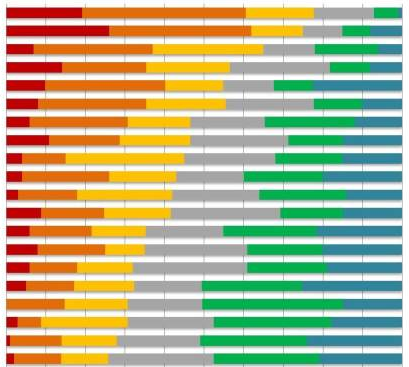
\includegraphics[width=0.3\linewidth]{figures/analysis/stacked-bar-without-baseline} }}%
  \qquad
  \subfloat[.. with baseline]{{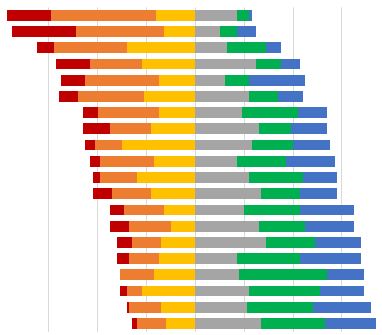
\includegraphics[width=0.3\linewidth]{figures/analysis/stacked-bar-with-baseline} }}%
  \caption{Stacked bar charts can be ordered along a baseline or stretch to 100\% width to show the percentage-of-the-whole of each group~\parencite{Mann2017}~\parencite{Peltier2017}.}%
  \label{fig:analysis:stacked-bar-chart}
\end{figure}

Unlike a multi-set bar graph which displays bars side-by-side, stacked bar graphs segment their bars of multiple datasets on top of each other.
A baseline, as shown in figure~\ref{fig:analysis:stacked-bar-chart} might be modeled as two back-to-back multi-set bar graphs. A reordering would e.g.\ move one data set from the left side to the right side.
A stacked bar chart also expects \emph{tabular} data.

If the stacked bar chart has a baseline, often the algebraic sign of the numeric value defines the placement of the segment on the left or on the right side.
Table~\ref{tab:analysis:stacked-bar-chart:interactions} shows possible interactions, including the highlighting of a data point, a change of color mapping or a reordering of the baseline.
% \conceptTable{Tabular data, multiple date sets as series}{Size, shape, orientation.}{Color, position, texture.}

\begin{table}[H]
  \caption{Plausible interactions for stacked bar charts.}%
  \label{tab:analysis:stacked-bar-chart:interactions}
  \begin{tabularx}{\linewidth}{lXX}
    \bf Category & \bf Description & \bf Required information \\
    \hline
    \bf Select & Highlight a bar & id of data point \\
    \bf Encode & Change colour mapping & id of data series + colour \\
    \bf Reconfigure & Sort by attribute & name of data attribute \\
    \bf Reconfigure & Specify stacking order & ordered list of ids of data series \\
    \bf Reconfigure & Flip data series & list of ids of data series \\
    \bf Filter & Hide a data series & id of data series \\
  \end{tabularx}
\end{table}


\subsection{Hierarchical visualizations}

\begin{figure}
  \centering
  \subfloat[Tree map]{{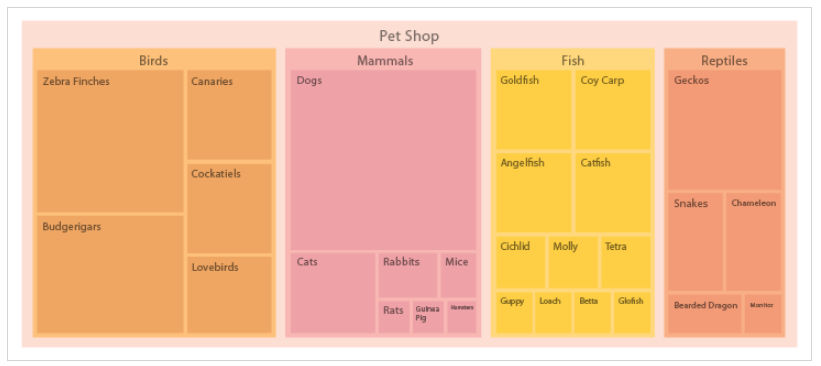
\includegraphics[width=0.4\linewidth]{figures/analysis/treemap} }}%
  \qquad
  \subfloat[Sunburst diagram]{{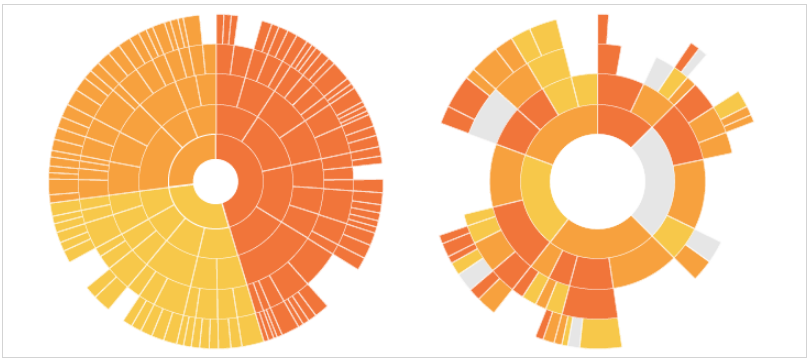
\includegraphics[width=0.4\linewidth]{figures/analysis/sunburst} }}%
  \caption{Tree maps and sunburst diagrams are ideal to show hierarchies~\parencite{VisualizationCatalogue2017}.}%
  \label{fig:analysis:hierarchies}
\end{figure}

Tree maps are great to show hierarchical data without ever exceeding the available screen.
Each data point is represented as a tile.
Unlike a treemap a hierarchical ring diagram or sunburst diagram shows each level of the underlying tree as a series of rings.

Therefore, both treemap and ring diagram expect \emph{hierarchic} data.
Typically, each node will have at least one continuous value that can be used as input for the tiling algorithm or layout algorithm respectively.
Additionally, each node can encode more attributes by colour.

As these visualization techniques are about hierarchies, the visible, maximal depth of the tree may be increased or decreased.
Again, interactions could include a highlighting of data points and a change of color encoding.
Both visualizations may show only a subtree.
E.g.\ a click on a box in the treemap opens another treemap focused on the subtree.
Similarly, a click on a slice of the ring would surround the most external ring with the child nodes of the parent node.
Table~\ref{tab:analysis:hierarchies:interactions} gives a more comprehensive list of interactions.

% \conceptTable{Tree, each feature has a value for layouting.}{Position, Size, shape, orientation.}{Color, texture.}

\begin{table}[H]
  \caption{Plausible interactions for hierarchical visualizations.}%
  \label{tab:analysis:hierarchies:interactions}
  \begin{tabularx}{\linewidth}{lXX}
    \bf Category & \bf Description & \bf Required information \\
    \hline
    Select & Highlight a node & id of data point \\
    Explore & Use another node as root of the visible tree & id of data point \\
    Encode & Change mapping of category to colour & id of data series + colour \\
    Reconfigure & Change data attribute used for layout & name of data attribute \\
    Reconfigure & Sort by attribute & name of data attribute \\
    Reconfigure & Specify order & ordered list of ids of data points \\
    Abstract/Elaborate & Specify maximum depth of visible tree & number of hierarchy levels \\
  \end{tabularx}
\end{table}

\subsection{Geographic Data Visualizations}

\begin{figure}
  \centering
  \subfloat[Choropleth map]{{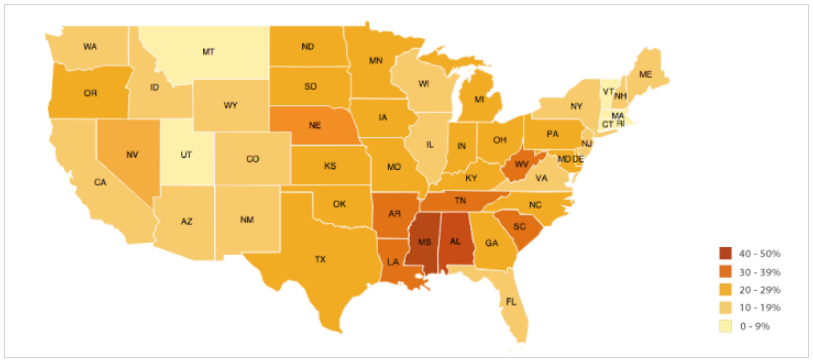
\includegraphics[width=0.4\linewidth]{figures/analysis/choropleth-map} }}%
  \qquad
  \subfloat[Flow map]{{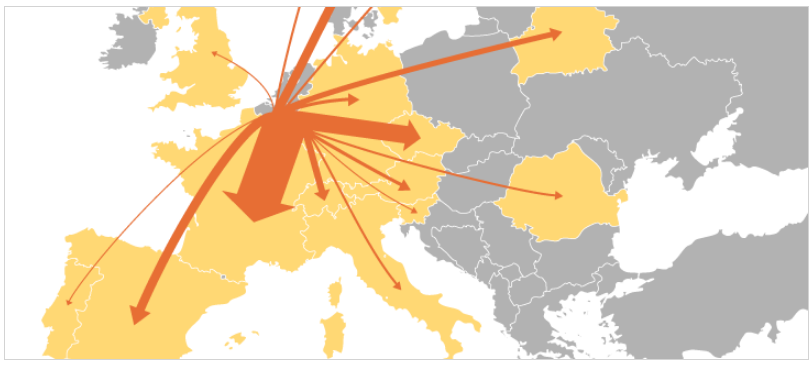
\includegraphics[width=0.4\linewidth]{figures/analysis/flow-map} }}%
  \caption{Choropleth maps focus on a density while flow maps show a migration of data~\parencite{VisualizationCatalogue2017}.}%
  \label{fig:analysis:geographical}
\end{figure}

Choropleth maps and flow maps are thematic maps to visualize geographic data.
Size, position and shape of a data point is determined by its geometry.
Choropleth maps encode a continuous data attribute with relative values in the color of each region.
Flow maps may display relationships between features, a data value defining the size, colour, direction or shape of each arrow.
Figure~\ref{fig:analysis:geographical} shows an example for each technique.

Non-geographic data may be given in a \emph{tabular} form, assigned to each geographic feature.
In contrast to tabular data, a flow map expects relationships between geographic features.
Thus, it also expects \emph{relational} data in form of a graph

% \conceptTable{Graph data with edges, each feature has geometry data.}{Position, Size, shape, orientation.}{Color, texture.}

\begin{table}[H]
  \caption{Plausible interactions for geographic visualizations.}%
  \label{tab:analysis:geographical:interactions}
  \begin{tabularx}{\linewidth}{lXX}
    \bf Category & \bf Description & \bf Required information \\
    \hline
    Select & Highlight a feature & id of data point \\
    Explore & Move viewport & latitude and longitude of viewpoint \\
    Explore & Zoom in, zoom out & zoom factor \\
    Encode & Change shape of marker & data id  shape \\
    Encode & Change mapping of category to colour & id of data series + colour \\
    Encode & Change colour function & value + colour \\
    Encode & Change data attribute used for colour & name of data attribute \\
    Connect & Show relations of a feature & id of data point  \\
    Abstract/Elaborate & Change granularity of displayed regions & number of hierarchy levels \\
  \end{tabularx}
\end{table}

\textbf{Temporal Data Visualizations}
\begin{figure}
  \centering
  \subfloat[Calendar]{{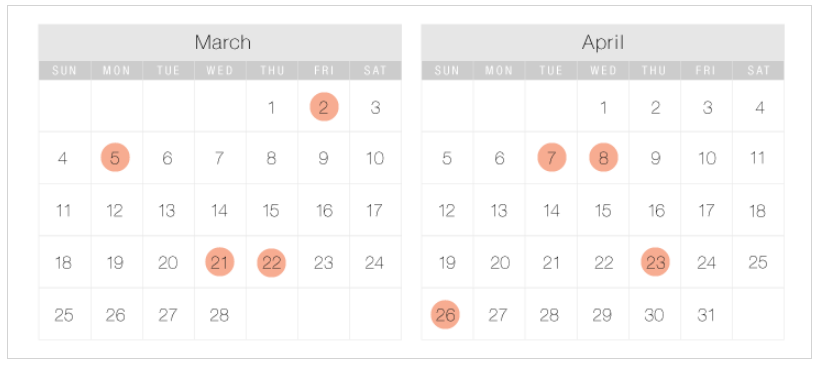
\includegraphics[width=0.4\linewidth]{figures/analysis/calendar} }}%
  \qquad
  \subfloat[Gantt chart]{{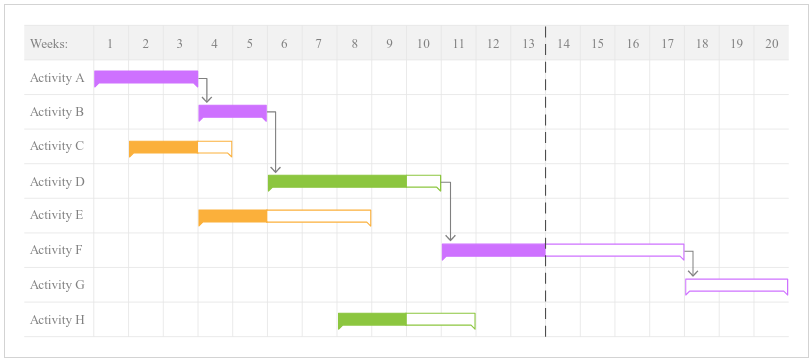
\includegraphics[width=0.4\linewidth]{figures/analysis/gantt-chart} }}%
  \caption{Similar to a calendar, a gantt chart shows activities and the progress along a time line~\parencite{VisualizationCatalogue2017}.}%
  \label{fig:analysis:temporal}
\end{figure}

Activity diagrams, like calendars and gantt charts, and timelines are temporal visualizations.
Gantt charts and timelines have in common that each feature is represented as a rectangle, with the duration of the feature mapped to size and position.
A calendar, as shown in Figure~\ref{fig:analysis:temporal}, may show the event as a single marker for brevity.
Calendars and gantt charts could not only read the data from the data source, but also add new features to the data set or update metadata of a feature, e.g.\ the progress of the activity.
Calendars and gantt charts expect \emph{tabular} data, although data points might reoccur on a regular schedule.
So some data points, i.e.\ events, might repeat infinitely.
A very common interaction is the filtering of the data set by selecting an interval over a timeline visualization, e.g. by dragging the mouse from left to right.
A more comprehensive list is shown in Table~\ref{tab:analysis:temporal:interactions}.

% \conceptTable{Temporal data, each feature has a time interval.}{Position, Size, orientation.}{Color, shape, texture.}

\begin{table}
  \caption{Interactions for temporal visualizations.}%
  \label{tab:analysis:temporal:interactions}
  \begin{tabularx}{\linewidth}{lXX}
    \bf Category & \bf Description & \bf Required information \\
    \hline
    Select & Highlight a feature & id of data point \\
    Explore & Show a different period of dates & start and end datetime \\
    Explore & Show a different time interval & start and end hour\\
    Encode & Change color of categories or activities & id of data series + colour \\
    Encode & Change data attribute used for colour & data attribute \\
    Filter & Remove a calendar or a category & id of data series \\
    Filter & Filter data set by time interval & upper and lower limit \\
  \end{tabularx}
\end{table}

% \section{Multiple View Interactions}\label{sec:analysis:examples:multiple}

% This section covers examples of multiple data visualizations.
% Combination of views are often very specific to certain use cases.
% That's why the examples in this section are tied to a use case in contrast to the more generic examples in Section~\ref{sec:analysis:examples}.


% \subsection{Detail view and Mini View}
% \begin{figure}
%   \centering
%   \subfloat[Detail view]{ 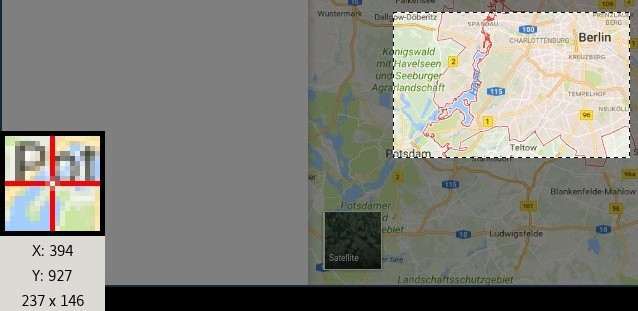
\includegraphics[width=0.4\linewidth]{figures/analysis/detail-view} }%
%   \qquad
%   \subfloat[Mini view]{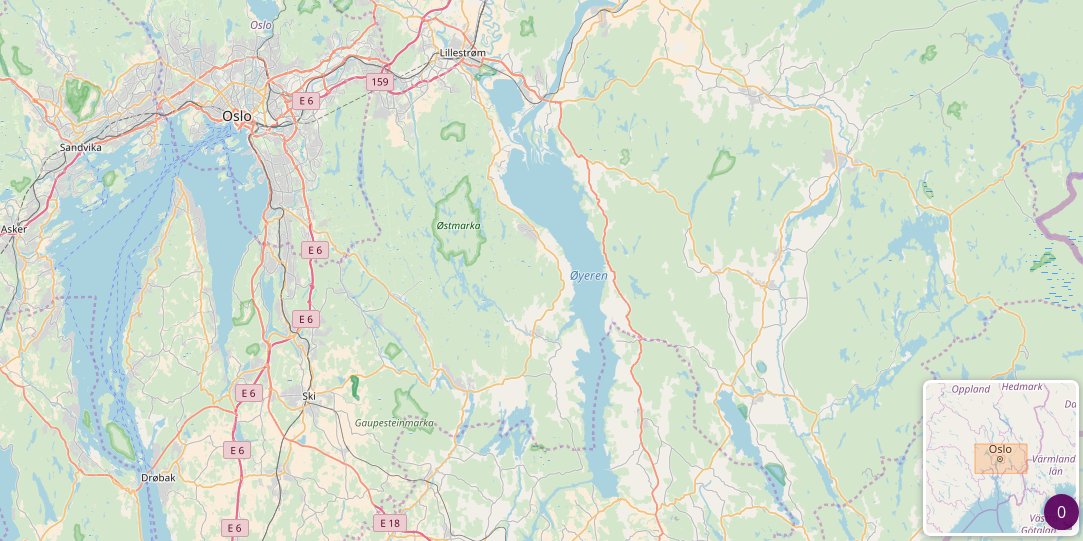
\includegraphics[width=0.4\linewidth]{figures/analysis/mini-view}}%
%   \caption{
%     The screenshot-tool ``Shutter'' shows a magnified detail view of the area around the mouse cursor in the lower left corner of the screen.
%   The opposite approach is e.g.\ ``Leaflet-Minimap'' that shows the map at a larger scale in the lower right.
%   }
%   \label{fig:analysis:detail}
% \end{figure}

% Detail views show a magnification of the surrounding area of a cursor in a secondary view.
% The resolution of the primary view is too high for the user to distinguish individual pixels.
% The detail view helps to select items.
% Popular use cases are screenshot tools, as seen on the left in Figure~\ref{fig:analysis:detail}, or image processing application.

% The opposite of a detail view is the mini view.
% You can see an example on the right side of Figure~\ref{fig:analysis:detail}.
% This secondary view shows a larger surrounding of the primary view, if the primary view shows only a section of the entire space.
% Use cases are geographic visualizations and therefore the expected data structure is a map with coordinates of the viewpoint and a zoom factor for each view.

% \begin{table}[H]
%   \caption{Plausible interactions for detail and mini views.}%
%   \label{fig:analysis:detail:interactions}
%   \begin{tabularx}{\linewidth}{lXX}
%     \bf Category & \bf Description & \bf Required information \\
%     \hline
%     Explore & Move secondary viewpoint & Latitude + Longitude \\
%     Explore & Move primary viewpoint through secondary view & Latitude + Longitude \\
%     Explore & Accelerate scrolling via secondary view & Zoom factor \\
%   \end{tabularx}
% \end{table}


% \subsection{Timeline}

% \begin{figure}
%   \centering
%     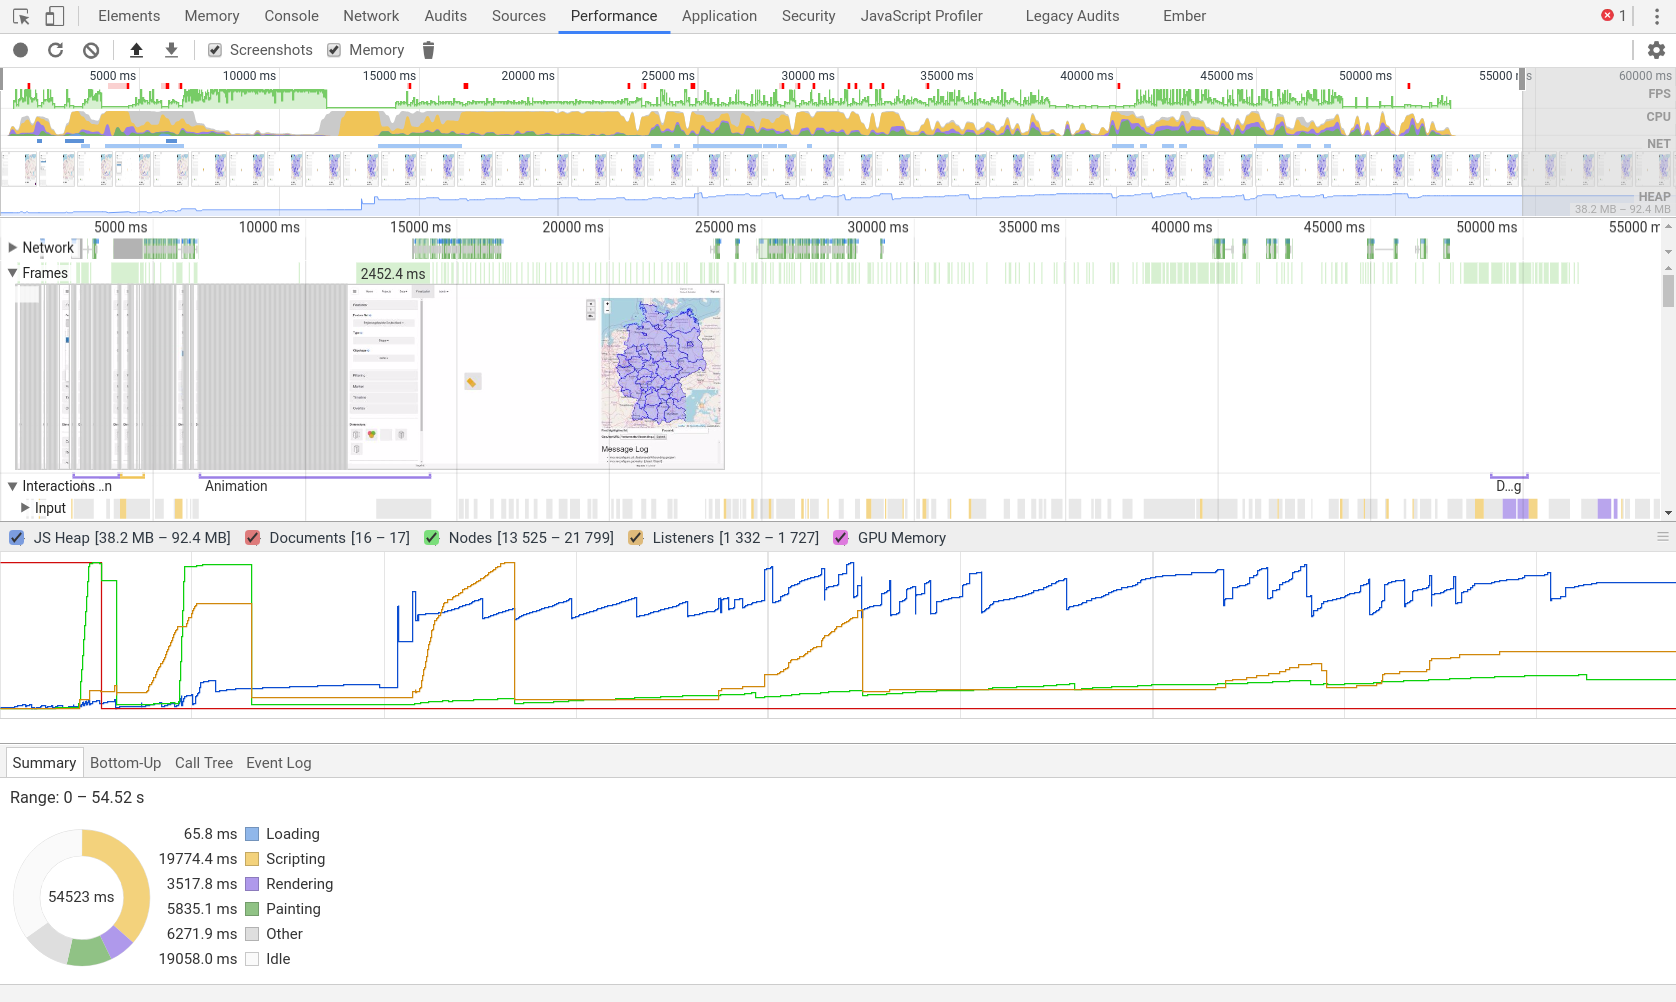
\includegraphics[width=\linewidth]{figures/analysis/profiler}
%   \caption{Multiple views of Chromium's runtime analysis tool can be focused on a selected time span.}
%   \label{fig:analysis:timeline}
% \end{figure}
% Figure~\ref{fig:analysis:timeline} shows the runtime analysis of the Chromium browser.
% Multiple views show different granularities of the same data.
% At the top, the entire profiling time frame is visualized, with a screenshot of one step in the middle.
% The development of memory is displayed on the third row while a summary is on the bottom.
% The user can select a window on the top line and the data for the other views is reduced according to the selected window.
% A multiple visualization like that expects \emph{temporal} data.

% \begin{table}[H]
%   \caption{Plausible interactions for timelines.}%
%   \label{fig:analysis:timeline:interactions}
%   \begin{tabularx}{\linewidth}{lXX}
%     \bf Category & \bf Description & \bf Required information \\
%     \hline
%     Filter & Filter data by time span & Upper and lower limit \\
%     Select & Display screenshot a certain time & Timestamp  \\
%   \end{tabularx}
% \end{table}


